% Additional results (moved from main.tex appendix to the supplement).
\section{Additional Results}
\label{app:additional}

\Cref{fig:designs} extends \Cref{tab:e2} to five budgets, from $m=n/2$ to
$m=8n$, and \Cref{fig:ci} reports the interval coverage, interval widths,
and distinctiveness recovery summarized in \Cref{sec:exp-ci}.

\begin{figure}[!ht]
  \centering
  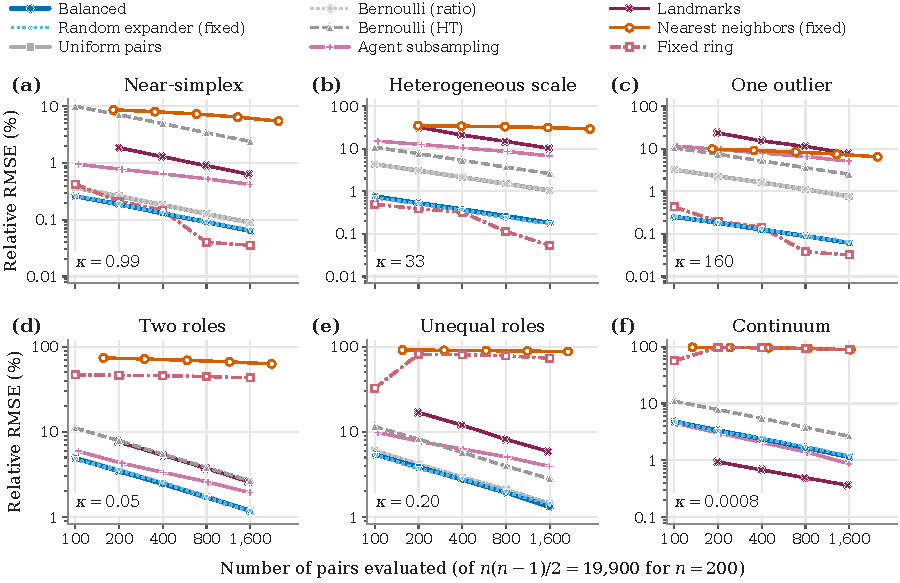
\includegraphics[width=\textwidth]{figures/fig_designs.pdf}
  \caption{\textbf{Error of every design across budgets.} Relative RMSE
  against the number of pairs evaluated for the six synthetic families of
  \Cref{tab:synthetic} ($n=200$; root mean square over three tables per
  family; \Cref{tab:e2} is the slice $m=2n$). Each design is plotted at the
  number of pairs it actually evaluates: symmetrized nearest-neighbor graphs
  use between $m$ and $2m$, and landmarks never fewer than $n-1=199$. The
  balanced (round-robin) design and a fixed random expander coincide in
  every family, as \Cref{thm:balanced} predicts for a regular graph drawn
  independently of the labels; where two designs coincide, the second
  (expander, Bernoulli (ratio)) is drawn dotted on top of the first. Uniform and Bernoulli (ratio) sampling
  overlap in every panel and coincide with the balanced design (drawn
  behind it) only when $\kappa\approx 0$. The nearest-neighbor
  graph, which is built from the table itself, is biased in every family,
  and its error barely decreases with $m$. The fixed ring is strongly biased only in
  the bottom row, where labels follow the generator's ordering; in the top
  row its expected squared error equals the balanced variance
  (\Cref{thm:balanced}), and the points are single realizations on three tables.}
  \label{fig:designs}
\end{figure}

\begin{figure}[!ht]
  \centering
  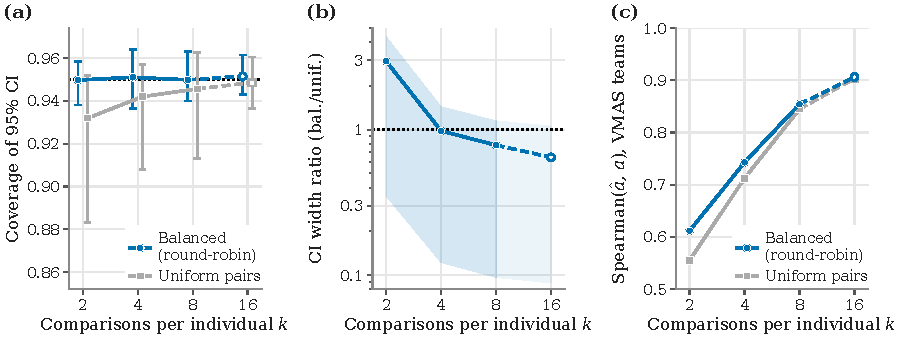
\includegraphics[width=\textwidth]{figures/fig_ci.pdf}
  \caption{\textbf{Error bars and distinctiveness from sparse balanced
  designs.} CI denotes a $95\%$ confidence interval. Results over $26$ tables: six synthetic families ($n=200$), the
  $128$-model population, and $19$ VMAS tables (four trained teams, $14$
  one-outlier and two-group variants, and one untrained $n=100$ team), with
  $2{,}000$ draws per table and
  $k$. At $k=16$ the design needs $n-1\ge16$ rounds, so only the $13$ tables
  with $n\ge32$ enter (dashed segments, open markers). (a) Coverage of nominal $95\%$
  intervals. Balanced (round-robin) intervals treat the $k$ round means as a
  simple random sample without replacement from the $n-1$ rounds, with a
  $t_{k-1}$ quantile and finite-population correction $1-k/(n-1)$. Markers
  show the mean over tables, bars the range over tables, and the dotted
  line the nominal level. Balanced intervals average $0.950$--$0.952$
  coverage at every $k$, whereas Wald intervals from uniform pairs
  undercover, down to $0.88$ on the synthetic one-outlier table at $k=2$.
  (b) Median width ratio, balanced/uniform (band: range over tables,
  lighter at $k=16$; dotted: equal width). The median ratio is $2.96$, $0.98$, $0.78$, and
  $0.65$ at $k=2$, $4$, $8$, and~$16$. At $k=2$ the median balanced interval is wider
  because the $t_1$ quantile ($12.7$) is $6.5$ times the normal one. For
  $k\ge4$ balanced intervals are up to $11\times$ narrower when distinctiveness dominates
  (one-outlier table) and at most $1.44\times$ wider when $\kappa\approx0$.
  (c) Rank correlation between estimated and true distinctiveness $a_i$ on
  the VMAS teams ($19$ tables; $6$ at $k=16$): four comparisons per individual
  already give a mean Spearman correlation of $0.74$ (first $300$ draws per
  table).}
  \label{fig:ci}
\end{figure}

